\section{Bifurcation Theory}

Here in this section we will explore the ideas of the bifurcation theory in the dynamical systems. This is a very important topic since it can give explanation for some sudden change that we see in the nature (for example the type I and type II phase transition in the thermodynamics). We will study them with the following classification.

\subsubsection{A Quick Review}
Consider the following family of dynamical systems parameterized by one parameter $\alpha$. 
\[ \dot{x} = f(x,\alpha), \]
where $f:\R \times \R \to \R$, and $x,\alpha \in \R$. And assume $f(x_0,\alpha_0)=0$, thus for $\alpha=\alpha_0$ the point $x_0$ is an equilibrium point. Now we can do the linearization at the equilibrium point and determine the type of stability. Thus after linearization we will have
\[ \dot{x} = f_x(x_0,\alpha_0) (x-x_0). \]
By letting $\xi = x - x_0$ we can now write
\[ \dot{\xi} = f_x(0,\alpha_0) \xi. \]
This is a very simple ODE whose solution is the exponential function. Thus we will have
\begin{align*}
	f_x(x_0,\alpha_0) &< 0 \implies \text{$x_0$ is stable}.\\
	f_x(x_0,\alpha_0) &> 0 \implies \text{$x_0$ is unstable}.\\
	f_x(x_0,\alpha_0) &=0 \implies \text{more terms from the Taylor's series is needed. } 
\end{align*}
Another way of seeing this is the following figure. Note that we can still determine the type of stability by looking at the graph, despite the fact that in the classification above we have said that in that case more terms from the Taylor's series is needed. The point is that when we are looking at the graph, we automatically infer the higher order terms of the Taylor's series as well and that is why we arrive at the right conclusion often.
\begin{figure}[h!]
	\centering
	
	
	
	\tikzset{every picture/.style={line width=0.75pt}} %set default line width to 0.75pt        
	
	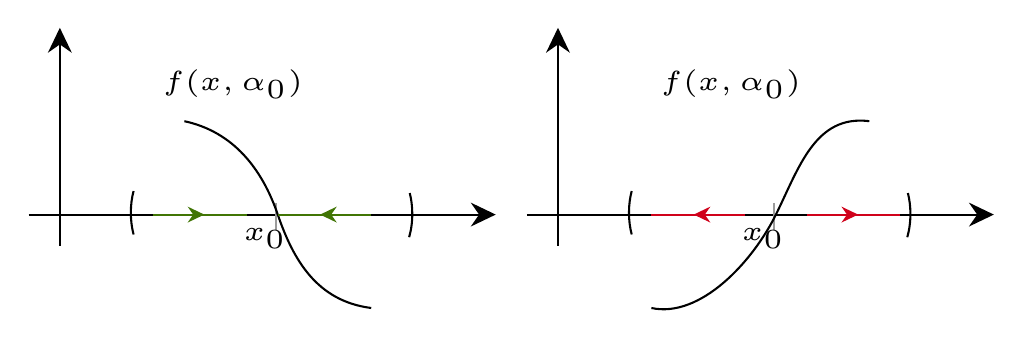
\begin{tikzpicture}[x=0.75pt,y=0.75pt,yscale=-1.5,xscale=1.5]
		%uncomment if require: \path (0,300); %set diagram left start at 0, and has height of 300
		
		%Straight Lines [id:da6141249148083039] 
		\draw    (80,150) -- (227,150) ;
		\draw [shift={(230,150)}, rotate = 180] [fill={rgb, 255:red, 0; green, 0; blue, 0 }  ][line width=0.08]  [draw opacity=0] (8.04,-3.86) -- (0,0) -- (8.04,3.86) -- (5.34,0) -- cycle    ;
		%Straight Lines [id:da4256457462457566] 
		\draw    (90,160) -- (90,93) ;
		\draw [shift={(90,90)}, rotate = 90] [fill={rgb, 255:red, 0; green, 0; blue, 0 }  ][line width=0.08]  [draw opacity=0] (8.04,-3.86) -- (0,0) -- (8.04,3.86) -- (5.34,0) -- cycle    ;
		%Shape: Arc [id:dp06425887483981807] 
		\draw  [draw opacity=0] (113.68,156.39) .. controls (113.12,154.26) and (112.8,151.89) .. (112.8,149.4) .. controls (112.8,146.92) and (113.11,144.56) .. (113.68,142.43) -- (122.8,149.4) -- cycle ; \draw   (113.68,156.39) .. controls (113.12,154.26) and (112.8,151.89) .. (112.8,149.4) .. controls (112.8,146.92) and (113.11,144.56) .. (113.68,142.43) ;  
		%Shape: Arc [id:dp36365112063998306] 
		\draw  [draw opacity=0] (202.39,143.08) .. controls (202.91,145.14) and (203.2,147.41) .. (203.2,149.8) .. controls (203.2,152.48) and (202.84,155.01) .. (202.19,157.26) -- (193.2,149.8) -- cycle ; \draw   (202.39,143.08) .. controls (202.91,145.14) and (203.2,147.41) .. (203.2,149.8) .. controls (203.2,152.48) and (202.84,155.01) .. (202.19,157.26) ;  
		%Straight Lines [id:da9959510519703285] 
		\draw [color={rgb, 255:red, 155; green, 155; blue, 155 }  ,draw opacity=1 ]   (159.4,146.2) -- (159.4,155) ;
		%Curve Lines [id:da23263506141610102] 
		\draw    (130,120) .. controls (145.8,123.4) and (155,135.4) .. (160,150) .. controls (165,164.6) and (172.6,177.8) .. (190,180) ;
		%Straight Lines [id:da06316055058145875] 
		\draw [color={rgb, 255:red, 65; green, 117; blue, 5 }  ,draw opacity=1 ]   (120,150) -- (150,150) ;
		\draw [shift={(136.4,150)}, rotate = 180] [fill={rgb, 255:red, 65; green, 117; blue, 5 }  ,fill opacity=1 ][line width=0.08]  [draw opacity=0] (5.36,-2.57) -- (0,0) -- (5.36,2.57) -- (3.56,0) -- cycle    ;
		%Straight Lines [id:da5497631725058023] 
		\draw [color={rgb, 255:red, 65; green, 117; blue, 5 }  ,draw opacity=1 ]   (190,150) -- (160,150) ;
		\draw [shift={(173.6,150)}, rotate = 360] [fill={rgb, 255:red, 65; green, 117; blue, 5 }  ,fill opacity=1 ][line width=0.08]  [draw opacity=0] (5.36,-2.57) -- (0,0) -- (5.36,2.57) -- (3.56,0) -- cycle    ;
		%Straight Lines [id:da09861653689071792] 
		\draw    (240,150) -- (387,150) ;
		\draw [shift={(390,150)}, rotate = 180] [fill={rgb, 255:red, 0; green, 0; blue, 0 }  ][line width=0.08]  [draw opacity=0] (8.04,-3.86) -- (0,0) -- (8.04,3.86) -- (5.34,0) -- cycle    ;
		%Straight Lines [id:da21639286510164335] 
		\draw    (250,160) -- (250,93) ;
		\draw [shift={(250,90)}, rotate = 90] [fill={rgb, 255:red, 0; green, 0; blue, 0 }  ][line width=0.08]  [draw opacity=0] (8.04,-3.86) -- (0,0) -- (8.04,3.86) -- (5.34,0) -- cycle    ;
		%Shape: Arc [id:dp8981115574458696] 
		\draw  [draw opacity=0] (273.68,156.39) .. controls (273.12,154.26) and (272.8,151.89) .. (272.8,149.4) .. controls (272.8,146.92) and (273.11,144.56) .. (273.68,142.43) -- (282.8,149.4) -- cycle ; \draw   (273.68,156.39) .. controls (273.12,154.26) and (272.8,151.89) .. (272.8,149.4) .. controls (272.8,146.92) and (273.11,144.56) .. (273.68,142.43) ;  
		%Shape: Arc [id:dp06952342542904488] 
		\draw  [draw opacity=0] (362.39,143.08) .. controls (362.91,145.14) and (363.2,147.41) .. (363.2,149.8) .. controls (363.2,152.48) and (362.84,155.01) .. (362.19,157.26) -- (353.2,149.8) -- cycle ; \draw   (362.39,143.08) .. controls (362.91,145.14) and (363.2,147.41) .. (363.2,149.8) .. controls (363.2,152.48) and (362.84,155.01) .. (362.19,157.26) ;  
		%Straight Lines [id:da1271782911650352] 
		\draw [color={rgb, 255:red, 155; green, 155; blue, 155 }  ,draw opacity=1 ]   (319.4,146.2) -- (319.4,155) ;
		%Curve Lines [id:da20362079394350396] 
		\draw    (280,180) .. controls (295.8,183.4) and (312.6,165) .. (320,150) .. controls (327.4,135) and (332.6,117.8) .. (350,120) ;
		%Straight Lines [id:da6324765334271558] 
		\draw [color={rgb, 255:red, 208; green, 2; blue, 27 }  ,draw opacity=1 ]   (330,150) -- (360,150) ;
		\draw [shift={(346.4,150)}, rotate = 180] [fill={rgb, 255:red, 208; green, 2; blue, 27 }  ,fill opacity=1 ][line width=0.08]  [draw opacity=0] (5.36,-2.57) -- (0,0) -- (5.36,2.57) -- (3.56,0) -- cycle    ;
		%Straight Lines [id:da3762166451314517] 
		\draw [color={rgb, 255:red, 208; green, 2; blue, 27 }  ,draw opacity=1 ]   (310,150) -- (280,150) ;
		\draw [shift={(293.6,150)}, rotate = 360] [fill={rgb, 255:red, 208; green, 2; blue, 27 }  ,fill opacity=1 ][line width=0.08]  [draw opacity=0] (5.36,-2.57) -- (0,0) -- (5.36,2.57) -- (3.56,0) -- cycle    ;
		
		% Text Node
		\draw (121,101.4) node [anchor=north west][inner sep=0.75pt]  [font=\tiny,xscale=2,yscale=2]  {$f( x,\alpha _{0})$};
		% Text Node
		\draw (147,152.4) node [anchor=north west][inner sep=0.75pt]  [font=\tiny,xscale=2,yscale=2]  {$x_{0}$};
		% Text Node
		\draw (281,101.4) node [anchor=north west][inner sep=0.75pt]  [font=\tiny,xscale=2,yscale=2]  {$f( x,\alpha _{0})$};
		% Text Node
		\draw (307,152.4) node [anchor=north west][inner sep=0.75pt]  [font=\tiny,xscale=2,yscale=2]  {$x_{0}$};
		
		
	\end{tikzpicture}
\end{figure}

It turns out that because of the smooth dependence of the function $f$ on both parameters, by sufficiently small enough perturbation of the parameter $\alpha$ from $\alpha_0$ the stability type of the equilibrium point will remain the same up to topological equivalence. For example in the figure below, the type of equilibrium point has remained the same (in this case stable equilibrium) with sufficiently small perturbation of parameter $\alpha$.

\begin{figure}[h!]
	\centering
	
	
	\tikzset{every picture/.style={line width=0.75pt}} %set default line width to 0.75pt        
	
	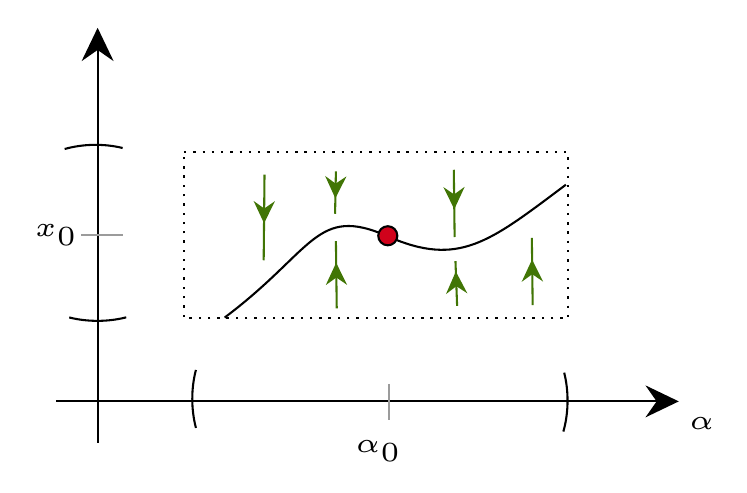
\begin{tikzpicture}[x=0.75pt,y=0.75pt,yscale=-2,xscale=2]
		%uncomment if require: \path (0,300); %set diagram left start at 0, and has height of 300
		
		%Curve Lines [id:da6170748878007859] 
		\draw    (280.6,129.8) .. controls (302.16,113.63) and (302.6,102.6) .. (319.8,110.2) .. controls (337,117.8) and (344.36,111.63) .. (362.8,97.8) ;
		%Straight Lines [id:da09861653689071792] 
		\draw    (240,150) -- (387,150) ;
		\draw [shift={(390,150)}, rotate = 180] [fill={rgb, 255:red, 0; green, 0; blue, 0 }  ][line width=0.08]  [draw opacity=0] (8.04,-3.86) -- (0,0) -- (8.04,3.86) -- (5.34,0) -- cycle    ;
		%Straight Lines [id:da21639286510164335] 
		\draw    (250,160) -- (250,63) ;
		\draw [shift={(250,60)}, rotate = 90] [fill={rgb, 255:red, 0; green, 0; blue, 0 }  ][line width=0.08]  [draw opacity=0] (8.04,-3.86) -- (0,0) -- (8.04,3.86) -- (5.34,0) -- cycle    ;
		%Shape: Arc [id:dp8981115574458696] 
		\draw  [draw opacity=0] (273.68,156.39) .. controls (273.12,154.26) and (272.8,151.89) .. (272.8,149.4) .. controls (272.8,146.92) and (273.11,144.56) .. (273.68,142.43) -- (282.8,149.4) -- cycle ; \draw   (273.68,156.39) .. controls (273.12,154.26) and (272.8,151.89) .. (272.8,149.4) .. controls (272.8,146.92) and (273.11,144.56) .. (273.68,142.43) ;  
		%Shape: Arc [id:dp06952342542904488] 
		\draw  [draw opacity=0] (362.39,143.08) .. controls (362.91,145.14) and (363.2,147.41) .. (363.2,149.8) .. controls (363.2,152.48) and (362.84,155.01) .. (362.19,157.26) -- (353.2,149.8) -- cycle ; \draw   (362.39,143.08) .. controls (362.91,145.14) and (363.2,147.41) .. (363.2,149.8) .. controls (363.2,152.48) and (362.84,155.01) .. (362.19,157.26) ;  
		%Straight Lines [id:da1271782911650352] 
		\draw [color={rgb, 255:red, 155; green, 155; blue, 155 }  ,draw opacity=1 ]   (320.2,145.8) -- (320.2,154.6) ;
		%Straight Lines [id:da39503739230709356] 
		\draw [color={rgb, 255:red, 155; green, 155; blue, 155 }  ,draw opacity=1 ]   (246,110) -- (256,110) ;
		%Shape: Arc [id:dp12989044576154574] 
		\draw  [draw opacity=0] (256.89,129.75) .. controls (254.79,130.29) and (252.46,130.59) .. (250.02,130.6) .. controls (247.58,130.6) and (245.26,130.31) .. (243.16,129.78) -- (250,120.8) -- cycle ; \draw   (256.89,129.75) .. controls (254.79,130.29) and (252.46,130.59) .. (250.02,130.6) .. controls (247.58,130.6) and (245.26,130.31) .. (243.16,129.78) ;  
		%Shape: Arc [id:dp6331916597674339] 
		\draw  [draw opacity=0] (242.06,89.2) .. controls (244.18,88.6) and (246.54,88.24) .. (249.03,88.2) .. controls (251.52,88.16) and (253.88,88.43) .. (256.02,88.96) -- (249.2,98.2) -- cycle ; \draw   (242.06,89.2) .. controls (244.18,88.6) and (246.54,88.24) .. (249.03,88.2) .. controls (251.52,88.16) and (253.88,88.43) .. (256.02,88.96) ;  
		%Shape: Rectangle [id:dp2141756481187609] 
		\draw  [dash pattern={on 0.84pt off 2.51pt}] (270.8,90) -- (363.4,90) -- (363.4,130) -- (270.8,130) -- cycle ;
		%Shape: Circle [id:dp6389280177413919] 
		\draw  [fill={rgb, 255:red, 208; green, 2; blue, 27 }  ,fill opacity=1 ] (317.6,110.1) .. controls (317.6,108.83) and (318.63,107.8) .. (319.9,107.8) .. controls (321.17,107.8) and (322.2,108.83) .. (322.2,110.1) .. controls (322.2,111.37) and (321.17,112.4) .. (319.9,112.4) .. controls (318.63,112.4) and (317.6,111.37) .. (317.6,110.1) -- cycle ;
		%Straight Lines [id:da3444362521363762] 
		\draw [color={rgb, 255:red, 65; green, 117; blue, 5 }  ,draw opacity=1 ]   (290.2,95.4) -- (290,116) ;
		\draw [shift={(290.09,107.1)}, rotate = 270.56] [fill={rgb, 255:red, 65; green, 117; blue, 5 }  ,fill opacity=1 ][line width=0.08]  [draw opacity=0] (5.36,-2.57) -- (0,0) -- (5.36,2.57) -- (3.56,0) -- cycle    ;
		%Straight Lines [id:da8243834750989563] 
		\draw [color={rgb, 255:red, 65; green, 117; blue, 5 }  ,draw opacity=1 ]   (307.4,94.6) -- (307.2,104.8) ;
		\draw [shift={(307.27,101.1)}, rotate = 271.12] [fill={rgb, 255:red, 65; green, 117; blue, 5 }  ,fill opacity=1 ][line width=0.08]  [draw opacity=0] (5.36,-2.57) -- (0,0) -- (5.36,2.57) -- (3.56,0) -- cycle    ;
		%Straight Lines [id:da11731949971207856] 
		\draw [color={rgb, 255:red, 65; green, 117; blue, 5 }  ,draw opacity=1 ]   (335.8,94.2) -- (336,110.4) ;
		\draw [shift={(335.92,103.7)}, rotate = 269.29] [fill={rgb, 255:red, 65; green, 117; blue, 5 }  ,fill opacity=1 ][line width=0.08]  [draw opacity=0] (5.36,-2.57) -- (0,0) -- (5.36,2.57) -- (3.56,0) -- cycle    ;
		%Straight Lines [id:da09921986693019402] 
		\draw [color={rgb, 255:red, 65; green, 117; blue, 5 }  ,draw opacity=1 ]   (354.6,110.6) -- (354.8,126.8) ;
		\draw [shift={(354.66,115.8)}, rotate = 89.29] [fill={rgb, 255:red, 65; green, 117; blue, 5 }  ,fill opacity=1 ][line width=0.08]  [draw opacity=0] (5.36,-2.57) -- (0,0) -- (5.36,2.57) -- (3.56,0) -- cycle    ;
		%Straight Lines [id:da6815749353841114] 
		\draw [color={rgb, 255:red, 65; green, 117; blue, 5 }  ,draw opacity=1 ]   (307.4,111.4) -- (307.6,127.6) ;
		\draw [shift={(307.46,116.6)}, rotate = 89.29] [fill={rgb, 255:red, 65; green, 117; blue, 5 }  ,fill opacity=1 ][line width=0.08]  [draw opacity=0] (5.36,-2.57) -- (0,0) -- (5.36,2.57) -- (3.56,0) -- cycle    ;
		%Straight Lines [id:da33325678105242607] 
		\draw [color={rgb, 255:red, 65; green, 117; blue, 5 }  ,draw opacity=1 ]   (336.2,116.2) -- (336.6,127) ;
		\draw [shift={(336.29,118.7)}, rotate = 87.88] [fill={rgb, 255:red, 65; green, 117; blue, 5 }  ,fill opacity=1 ][line width=0.08]  [draw opacity=0] (5.36,-2.57) -- (0,0) -- (5.36,2.57) -- (3.56,0) -- cycle    ;
		
		% Text Node
		\draw (391,152.4) node [anchor=north west][inner sep=0.75pt]  [font=\tiny,xscale=2,yscale=2]  {$\alpha $};
		% Text Node
		\draw (310.6,158) node [anchor=north west][inner sep=0.75pt]  [font=\tiny,xscale=2,yscale=2]  {$\alpha _{0}$};
		% Text Node
		\draw (233.4,106) node [anchor=north west][inner sep=0.75pt]  [font=\tiny,xscale=2,yscale=2]  {$x_{0}$};
		
		
	\end{tikzpicture}
\end{figure}

However, when $f_x(x_0,\alpha_0) = 0$, then it is possible that any perturbation of parameter $\alpha$ leads to the emergence or disappearance of a new type of equilibrium point, in which we say we have a \emph{bifurcation}. 


\subsection{Intuitive Explanation of Bifurcation}
In this section we will cover the intuitive explanation behind the notion of bifurcation and different types, and the next section we will cover the theory behind it and discuss the topological normal forms.
\subsubsection{Fold (Saddle-Note) Bifurcation}
The fold bifurcation is one of the simple type bifurcations where a saddle and a node emerges from blue sky as we vary the parameter $\alpha$. Following the line of reasoning from the section above, assume $f(x,\alpha_0)$ looks like the following in the neighborhood of the point $x_0$.

\begin{figure}[h!]
	\centering
	
	
	\tikzset{every picture/.style={line width=0.75pt}} %set default line width to 0.75pt        
	
	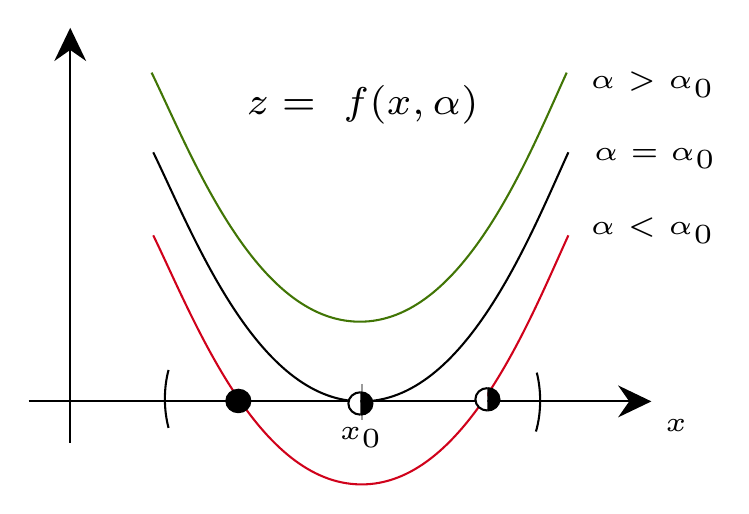
\begin{tikzpicture}[x=0.75pt,y=0.75pt,yscale=-2,xscale=2]
		%uncomment if require: \path (0,300); %set diagram left start at 0, and has height of 300
		
		%Straight Lines [id:da8292925238312234] 
		\draw    (260,170) -- (407,170) ;
		\draw [shift={(410,170)}, rotate = 180] [fill={rgb, 255:red, 0; green, 0; blue, 0 }  ][line width=0.08]  [draw opacity=0] (8.04,-3.86) -- (0,0) -- (8.04,3.86) -- (5.34,0) -- cycle    ;
		%Straight Lines [id:da4216739662290636] 
		\draw    (270,180) -- (270,83) ;
		\draw [shift={(270,80)}, rotate = 90] [fill={rgb, 255:red, 0; green, 0; blue, 0 }  ][line width=0.08]  [draw opacity=0] (8.04,-3.86) -- (0,0) -- (8.04,3.86) -- (5.34,0) -- cycle    ;
		%Shape: Arc [id:dp699038034905521] 
		\draw  [draw opacity=0] (293.68,176.39) .. controls (293.12,174.26) and (292.8,171.89) .. (292.8,169.4) .. controls (292.8,166.92) and (293.11,164.56) .. (293.68,162.43) -- (302.8,169.4) -- cycle ; \draw   (293.68,176.39) .. controls (293.12,174.26) and (292.8,171.89) .. (292.8,169.4) .. controls (292.8,166.92) and (293.11,164.56) .. (293.68,162.43) ;  
		%Shape: Arc [id:dp6219095318590535] 
		\draw  [draw opacity=0] (382.39,163.08) .. controls (382.91,165.14) and (383.2,167.41) .. (383.2,169.8) .. controls (383.2,172.48) and (382.84,175.01) .. (382.19,177.26) -- (373.2,169.8) -- cycle ; \draw   (382.39,163.08) .. controls (382.91,165.14) and (383.2,167.41) .. (383.2,169.8) .. controls (383.2,172.48) and (382.84,175.01) .. (382.19,177.26) ;  
		%Straight Lines [id:da2967293738460952] 
		\draw [color={rgb, 255:red, 155; green, 155; blue, 155 }  ,draw opacity=1 ]   (340.2,165.8) -- (340.2,174.6) ;
		%Curve Lines [id:da816687814370975] 
		\draw    (290,110) .. controls (299.8,130.2) and (315,169.8) .. (340,170) .. controls (365,170.2) and (380.6,130.6) .. (390,110) ;
		%Curve Lines [id:da1828248268569701] 
		\draw [color={rgb, 255:red, 65; green, 117; blue, 5 }  ,draw opacity=1 ]   (289.6,90.8) .. controls (299.4,111) and (314.6,150.6) .. (339.6,150.8) .. controls (364.6,151) and (380.2,111.4) .. (389.6,90.8) ;
		%Curve Lines [id:da12443143725658534] 
		\draw [color={rgb, 255:red, 208; green, 2; blue, 27 }  ,draw opacity=1 ]   (290,130) .. controls (299.8,150.2) and (315,189.8) .. (340,190) .. controls (365,190.2) and (380.6,150.6) .. (390,130) ;
		%Shape: Arc [id:dp4533006591675346] 
		\draw  [draw opacity=0][fill={rgb, 255:red, 255; green, 255; blue, 255 }  ,fill opacity=1 ] (370.5,172.2) .. controls (370.5,172.2) and (370.5,172.2) .. (370.5,172.2) .. controls (370.5,172.2) and (370.5,172.2) .. (370.5,172.2) .. controls (368.9,172.2) and (367.6,170.99) .. (367.6,169.5) .. controls (367.6,168.01) and (368.9,166.8) .. (370.5,166.8) -- (370.5,169.5) -- cycle ; \draw   (370.5,172.2) .. controls (370.5,172.2) and (370.5,172.2) .. (370.5,172.2) .. controls (370.5,172.2) and (370.5,172.2) .. (370.5,172.2) .. controls (368.9,172.2) and (367.6,170.99) .. (367.6,169.5) .. controls (367.6,168.01) and (368.9,166.8) .. (370.5,166.8) ;  
		%Shape: Arc [id:dp3446049661439001] 
		\draw  [draw opacity=0][fill={rgb, 255:red, 0; green, 0; blue, 0 }  ,fill opacity=1 ] (370.5,166.8) .. controls (370.5,166.8) and (370.5,166.8) .. (370.5,166.8) .. controls (370.5,166.8) and (370.5,166.8) .. (370.5,166.8) .. controls (372.1,166.8) and (373.4,168.01) .. (373.4,169.5) .. controls (373.4,170.99) and (372.1,172.2) .. (370.5,172.2) -- (370.5,169.5) -- cycle ; \draw   (370.5,166.8) .. controls (370.5,166.8) and (370.5,166.8) .. (370.5,166.8) .. controls (370.5,166.8) and (370.5,166.8) .. (370.5,166.8) .. controls (372.1,166.8) and (373.4,168.01) .. (373.4,169.5) .. controls (373.4,170.99) and (372.1,172.2) .. (370.5,172.2) ;  
		
		%Shape: Arc [id:dp188610151324339] 
		\draw  [draw opacity=0][fill={rgb, 255:red, 255; green, 255; blue, 255 }  ,fill opacity=1 ] (339.9,173.2) .. controls (339.9,173.2) and (339.9,173.2) .. (339.9,173.2) .. controls (339.9,173.2) and (339.9,173.2) .. (339.9,173.2) .. controls (338.3,173.2) and (337,171.99) .. (337,170.5) .. controls (337,169.01) and (338.3,167.8) .. (339.9,167.8) -- (339.9,170.5) -- cycle ; \draw   (339.9,173.2) .. controls (339.9,173.2) and (339.9,173.2) .. (339.9,173.2) .. controls (339.9,173.2) and (339.9,173.2) .. (339.9,173.2) .. controls (338.3,173.2) and (337,171.99) .. (337,170.5) .. controls (337,169.01) and (338.3,167.8) .. (339.9,167.8) ;  
		%Shape: Arc [id:dp013442113203225858] 
		\draw  [draw opacity=0][fill={rgb, 255:red, 0; green, 0; blue, 0 }  ,fill opacity=1 ] (339.9,167.8) .. controls (339.9,167.8) and (339.9,167.8) .. (339.9,167.8) .. controls (339.9,167.8) and (339.9,167.8) .. (339.9,167.8) .. controls (341.5,167.8) and (342.8,169.01) .. (342.8,170.5) .. controls (342.8,171.99) and (341.5,173.2) .. (339.9,173.2) -- (339.9,170.5) -- cycle ; \draw   (339.9,167.8) .. controls (339.9,167.8) and (339.9,167.8) .. (339.9,167.8) .. controls (339.9,167.8) and (339.9,167.8) .. (339.9,167.8) .. controls (341.5,167.8) and (342.8,169.01) .. (342.8,170.5) .. controls (342.8,171.99) and (341.5,173.2) .. (339.9,173.2) ;  
		
		%Shape: Path Data [id:dp7134098593263796] 
		\draw  [fill={rgb, 255:red, 0; green, 0; blue, 0 }  ,fill opacity=1 ] (307.6,169.9) .. controls (307.6,168.41) and (308.9,167.2) .. (310.5,167.2) .. controls (312.1,167.2) and (313.4,168.41) .. (313.4,169.9) .. controls (313.4,171.39) and (312.1,172.6) .. (310.5,172.6) .. controls (308.9,172.6) and (307.6,171.39) .. (307.6,169.9) -- cycle ;
		
		% Text Node
		\draw (333.4,174.8) node [anchor=north west][inner sep=0.75pt]  [font=\tiny,xscale=2,yscale=2]  {$x_{0}$};
		% Text Node
		\draw (411.8,172.8) node [anchor=north west][inner sep=0.75pt]  [font=\tiny,xscale=2,yscale=2]  {$x$};
		% Text Node
		\draw (393.8,124.4) node [anchor=north west][inner sep=0.75pt]  [font=\tiny,xscale=2,yscale=2]  {$\alpha < \alpha_0$};
		% Text Node
		\draw (394.6,107.6) node [anchor=north west][inner sep=0.75pt]  [font=\tiny,xscale=2,yscale=2]  {$\alpha = \alpha_0$};
		% Text Node
		\draw (393.8,89.2) node [anchor=north west][inner sep=0.75pt]  [font=\tiny,xscale=2,yscale=2]  {$\alpha  >\alpha_0$};
		% Text Node
		\draw (311,92.4) node [anchor=north west][inner sep=0.75pt]  [font=\scriptsize,xscale=2,yscale=2]  {$z=\ f( x,\alpha )$};
		
		
	\end{tikzpicture}
\end{figure}

Then as we can clearly see, any small perturbation of $\alpha$ will lead ot emergence or disappearance of new equilibria out of blue sky. We can not intuitively say that the requirements for such a bifurcation is the followings
\begin{enumerate}[(i)]
	\item $f(x_0,\alpha_0) = 0$,
	\item $f_x(x_0,\alpha_0) = 0$,
	\item $f_\alpha(x_0, \alpha_0) \neq 0$,
	\item $f_{xx}(x_0,\alpha_0) = \neq 0$.
\end{enumerate}

It is also informative to look at the branching diagram on the $(\alpha-x)$ plane.

\begin{figure}[h!]
	\centering
	
	
	\tikzset{every picture/.style={line width=0.75pt}} %set default line width to 0.75pt        
	
	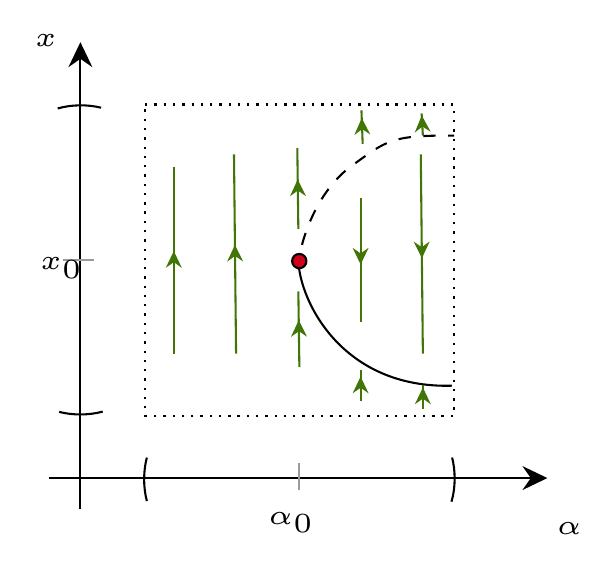
\begin{tikzpicture}[x=0.75pt,y=0.75pt,yscale=-1.5,xscale=1.5]
		%uncomment if require: \path (0,300); %set diagram left start at 0, and has height of 300
		
		%Straight Lines [id:da01424315752508698] 
		\draw    (280,170) -- (437,170) ;
		\draw [shift={(440,170)}, rotate = 180] [fill={rgb, 255:red, 0; green, 0; blue, 0 }  ][line width=0.08]  [draw opacity=0] (8.04,-3.86) -- (0,0) -- (8.04,3.86) -- (5.34,0) -- cycle    ;
		%Straight Lines [id:da8712066483107959] 
		\draw    (290,180) -- (290,33) ;
		\draw [shift={(290,30)}, rotate = 90] [fill={rgb, 255:red, 0; green, 0; blue, 0 }  ][line width=0.08]  [draw opacity=0] (8.04,-3.86) -- (0,0) -- (8.04,3.86) -- (5.34,0) -- cycle    ;
		%Shape: Arc [id:dp3120439738275269] 
		\draw  [draw opacity=0] (311.35,177.39) .. controls (310.78,175.26) and (310.47,172.89) .. (310.47,170.4) .. controls (310.47,167.92) and (310.78,165.56) .. (311.34,163.43) -- (320.47,170.4) -- cycle ; \draw   (311.35,177.39) .. controls (310.78,175.26) and (310.47,172.89) .. (310.47,170.4) .. controls (310.47,167.92) and (310.78,165.56) .. (311.34,163.43) ;  
		%Shape: Arc [id:dp31349560648241126] 
		\draw  [draw opacity=0] (409.39,163.41) .. controls (409.91,165.47) and (410.2,167.75) .. (410.2,170.13) .. controls (410.2,172.81) and (409.84,175.34) .. (409.19,177.6) -- (400.2,170.13) -- cycle ; \draw   (409.39,163.41) .. controls (409.91,165.47) and (410.2,167.75) .. (410.2,170.13) .. controls (410.2,172.81) and (409.84,175.34) .. (409.19,177.6) ;  
		%Straight Lines [id:da6244961621666105] 
		\draw [color={rgb, 255:red, 155; green, 155; blue, 155 }  ,draw opacity=1 ]   (360.2,165.13) -- (360.2,173.93) ;
		%Straight Lines [id:da6431539558000148] 
		\draw [color={rgb, 255:red, 155; green, 155; blue, 155 }  ,draw opacity=1 ]   (284.33,100) -- (294.33,100) ;
		%Shape: Arc [id:dp4718087034765315] 
		\draw  [draw opacity=0] (297.18,148.65) .. controls (295.01,149.24) and (292.59,149.56) .. (290.03,149.57) .. controls (287.6,149.57) and (285.28,149.28) .. (283.18,148.75) -- (290.02,139.77) -- cycle ; \draw   (297.18,148.65) .. controls (295.01,149.24) and (292.59,149.56) .. (290.03,149.57) .. controls (287.6,149.57) and (285.28,149.28) .. (283.18,148.75) ;  
		%Shape: Arc [id:dp17108201590896188] 
		\draw  [draw opacity=0] (282.7,51.28) .. controls (284.82,50.68) and (287.18,50.33) .. (289.67,50.28) .. controls (292.15,50.24) and (294.52,50.52) .. (296.65,51.04) -- (289.84,60.28) -- cycle ; \draw   (282.7,51.28) .. controls (284.82,50.68) and (287.18,50.33) .. (289.67,50.28) .. controls (292.15,50.24) and (294.52,50.52) .. (296.65,51.04) ;  
		%Shape: Rectangle [id:dp918196525444213] 
		\draw  [dash pattern={on 0.84pt off 2.51pt}] (310.8,50) -- (410,50) -- (410,150) -- (310.8,150) -- cycle ;
		%Straight Lines [id:da8323004033982035] 
		\draw [color={rgb, 255:red, 65; green, 117; blue, 5 }  ,draw opacity=1 ]   (380,80) -- (380,120) ;
		\draw [shift={(380,101.4)}, rotate = 270] [fill={rgb, 255:red, 65; green, 117; blue, 5 }  ,fill opacity=1 ][line width=0.08]  [draw opacity=0] (5.36,-2.57) -- (0,0) -- (5.36,2.57) -- (3.56,0) -- cycle    ;
		%Straight Lines [id:da47989466439408535] 
		\draw [color={rgb, 255:red, 65; green, 117; blue, 5 }  ,draw opacity=1 ]   (360,110) -- (360.33,134.33) ;
		\draw [shift={(360.13,119.27)}, rotate = 89.22] [fill={rgb, 255:red, 65; green, 117; blue, 5 }  ,fill opacity=1 ][line width=0.08]  [draw opacity=0] (5.36,-2.57) -- (0,0) -- (5.36,2.57) -- (3.56,0) -- cycle    ;
		%Curve Lines [id:da9034850510386916] 
		\draw    (360,100) .. controls (360.33,113) and (374,141.33) .. (409.33,140.33) ;
		%Curve Lines [id:da4103251770904497] 
		\draw  [dash pattern={on 4.5pt off 4.5pt}]  (360,103) .. controls (360,94.89) and (365.67,78) .. (377.13,69.72) .. controls (388.59,61.45) and (389.76,59.87) .. (410,60) ;
		%Shape: Circle [id:dp5048859507489949] 
		\draw  [fill={rgb, 255:red, 208; green, 2; blue, 27 }  ,fill opacity=1 ] (358,100.3) .. controls (358,99.03) and (359.03,98) .. (360.3,98) .. controls (361.57,98) and (362.6,99.03) .. (362.6,100.3) .. controls (362.6,101.57) and (361.57,102.6) .. (360.3,102.6) .. controls (359.03,102.6) and (358,101.57) .. (358,100.3) -- cycle ;
		%Straight Lines [id:da86776080159781] 
		\draw [color={rgb, 255:red, 65; green, 117; blue, 5 }  ,draw opacity=1 ]   (399.33,66) -- (400,130) ;
		\draw [shift={(399.68,99.4)}, rotate = 269.4] [fill={rgb, 255:red, 65; green, 117; blue, 5 }  ,fill opacity=1 ][line width=0.08]  [draw opacity=0] (5.36,-2.57) -- (0,0) -- (5.36,2.57) -- (3.56,0) -- cycle    ;
		%Straight Lines [id:da4088704269971215] 
		\draw [color={rgb, 255:red, 65; green, 117; blue, 5 }  ,draw opacity=1 ]   (380,135.33) -- (380,145.33) ;
		\draw [shift={(380,137.43)}, rotate = 90] [fill={rgb, 255:red, 65; green, 117; blue, 5 }  ,fill opacity=1 ][line width=0.08]  [draw opacity=0] (5.36,-2.57) -- (0,0) -- (5.36,2.57) -- (3.56,0) -- cycle    ;
		%Straight Lines [id:da8093137611981749] 
		\draw [color={rgb, 255:red, 65; green, 117; blue, 5 }  ,draw opacity=1 ]   (359.67,64) -- (360,90) ;
		\draw [shift={(359.8,74.1)}, rotate = 89.27] [fill={rgb, 255:red, 65; green, 117; blue, 5 }  ,fill opacity=1 ][line width=0.08]  [draw opacity=0] (5.36,-2.57) -- (0,0) -- (5.36,2.57) -- (3.56,0) -- cycle    ;
		%Straight Lines [id:da8832222987750873] 
		\draw [color={rgb, 255:red, 65; green, 117; blue, 5 }  ,draw opacity=1 ]   (380.27,51.87) -- (380.67,62.67) ;
		\draw [shift={(380.36,54.37)}, rotate = 87.88] [fill={rgb, 255:red, 65; green, 117; blue, 5 }  ,fill opacity=1 ][line width=0.08]  [draw opacity=0] (5.36,-2.57) -- (0,0) -- (5.36,2.57) -- (3.56,0) -- cycle    ;
		%Straight Lines [id:da17190568556425267] 
		\draw [color={rgb, 255:red, 65; green, 117; blue, 5 }  ,draw opacity=1 ]   (339.33,66) -- (340,130) ;
		\draw [shift={(339.64,95.1)}, rotate = 89.4] [fill={rgb, 255:red, 65; green, 117; blue, 5 }  ,fill opacity=1 ][line width=0.08]  [draw opacity=0] (5.36,-2.57) -- (0,0) -- (5.36,2.57) -- (3.56,0) -- cycle    ;
		%Straight Lines [id:da9753084599520274] 
		\draw [color={rgb, 255:red, 65; green, 117; blue, 5 }  ,draw opacity=1 ]   (400,140) -- (400,147.67) ;
		\draw [shift={(400,140.93)}, rotate = 90] [fill={rgb, 255:red, 65; green, 117; blue, 5 }  ,fill opacity=1 ][line width=0.08]  [draw opacity=0] (5.36,-2.57) -- (0,0) -- (5.36,2.57) -- (3.56,0) -- cycle    ;
		%Straight Lines [id:da01390022727383422] 
		\draw [color={rgb, 255:red, 65; green, 117; blue, 5 }  ,draw opacity=1 ]   (399.6,52.87) -- (400,60) ;
		\draw [shift={(399.64,53.54)}, rotate = 86.79] [fill={rgb, 255:red, 65; green, 117; blue, 5 }  ,fill opacity=1 ][line width=0.08]  [draw opacity=0] (5.36,-2.57) -- (0,0) -- (5.36,2.57) -- (3.56,0) -- cycle    ;
		%Straight Lines [id:da6113531905417322] 
		\draw [color={rgb, 255:red, 65; green, 117; blue, 5 }  ,draw opacity=1 ]   (320,70) -- (320,130) ;
		\draw [shift={(320,97.1)}, rotate = 90] [fill={rgb, 255:red, 65; green, 117; blue, 5 }  ,fill opacity=1 ][line width=0.08]  [draw opacity=0] (5.36,-2.57) -- (0,0) -- (5.36,2.57) -- (3.56,0) -- cycle    ;
		
		% Text Node
		\draw (441,182.4) node [anchor=north west][inner sep=0.75pt]  [font=\tiny,xscale=2,yscale=2]  {$\alpha $};
		% Text Node
		\draw (348.27,179) node [anchor=north west][inner sep=0.75pt]  [font=\tiny,xscale=2,yscale=2]  {$\alpha _{0}$};
		% Text Node
		\draw (275.07,97.33) node [anchor=north west][inner sep=0.75pt]  [font=\tiny,xscale=2,yscale=2]  {$x_{0}$};
		% Text Node
		\draw (273.4,25.67) node [anchor=north west][inner sep=0.75pt]  [font=\tiny,xscale=2,yscale=2]  {$x$};
		
		
	\end{tikzpicture}
\end{figure}


\subsubsection{Transcritical Bifurcation}
Another possible way that the function $f(x,\alpha)$ might change in the neighborhood of $x_0$ is the following diagram.

\begin{figure}[h!]
	\centering
	
	
	\tikzset{every picture/.style={line width=0.75pt}} %set default line width to 0.75pt        
	
	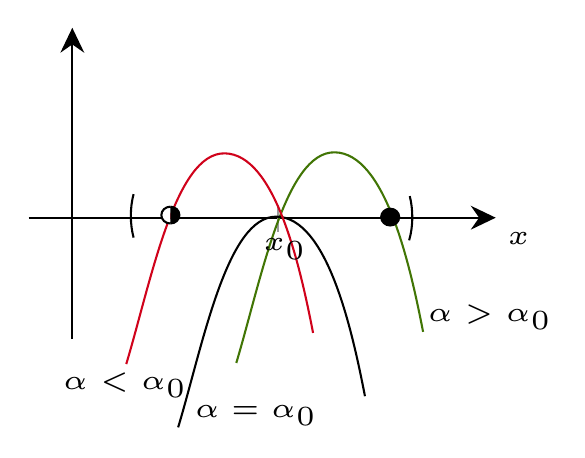
\begin{tikzpicture}[x=0.75pt,y=0.75pt,yscale=-1.5,xscale=1.5]
		%uncomment if require: \path (0,300); %set diagram left start at 0, and has height of 300
		
		%Straight Lines [id:da9186525400885985] 
		\draw    (197,80.67) -- (344,80.67) ;
		\draw [shift={(347,80.67)}, rotate = 180] [fill={rgb, 255:red, 0; green, 0; blue, 0 }  ][line width=0.08]  [draw opacity=0] (8.04,-3.86) -- (0,0) -- (8.04,3.86) -- (5.34,0) -- cycle    ;
		%Straight Lines [id:da6050428608083982] 
		\draw    (211,119.67) -- (211,22.67) ;
		\draw [shift={(211,19.67)}, rotate = 90] [fill={rgb, 255:red, 0; green, 0; blue, 0 }  ][line width=0.08]  [draw opacity=0] (8.04,-3.86) -- (0,0) -- (8.04,3.86) -- (5.34,0) -- cycle    ;
		%Shape: Arc [id:dp7703979857909888] 
		\draw  [draw opacity=0] (230.68,87.06) .. controls (230.12,84.92) and (229.8,82.56) .. (229.8,80.07) .. controls (229.8,77.58) and (230.11,75.22) .. (230.68,73.1) -- (239.8,80.07) -- cycle ; \draw   (230.68,87.06) .. controls (230.12,84.92) and (229.8,82.56) .. (229.8,80.07) .. controls (229.8,77.58) and (230.11,75.22) .. (230.68,73.1) ;  
		%Shape: Arc [id:dp5582597037845276] 
		\draw  [draw opacity=0] (319.39,73.74) .. controls (319.91,75.81) and (320.2,78.08) .. (320.2,80.47) .. controls (320.2,83.14) and (319.84,85.68) .. (319.19,87.93) -- (310.2,80.47) -- cycle ; \draw   (319.39,73.74) .. controls (319.91,75.81) and (320.2,78.08) .. (320.2,80.47) .. controls (320.2,83.14) and (319.84,85.68) .. (319.19,87.93) ;  
		%Straight Lines [id:da044005185629654164] 
		\draw [color={rgb, 255:red, 155; green, 155; blue, 155 }  ,draw opacity=1 ]   (277.2,76.47) -- (277.2,85.27) ;
		%Curve Lines [id:da14642227911662364] 
		\draw [color={rgb, 255:red, 65; green, 117; blue, 5 }  ,draw opacity=1 ]   (263.67,127.33) .. controls (271.67,100.67) and (279.33,59.33) .. (295.33,59.67) .. controls (311.33,60) and (319.33,95) .. (323.67,117.33) ;
		%Shape: Path Data [id:dp9638586133208085] 
		\draw  [fill={rgb, 255:red, 0; green, 0; blue, 0 }  ,fill opacity=1 ] (310.2,80.47) .. controls (310.2,78.98) and (311.5,77.77) .. (313.1,77.77) .. controls (314.7,77.77) and (316,78.98) .. (316,80.47) .. controls (316,81.96) and (314.7,83.17) .. (313.1,83.17) .. controls (311.5,83.17) and (310.2,81.96) .. (310.2,80.47) -- cycle ;
		%Curve Lines [id:da7744283987524179] 
		\draw [color={rgb, 255:red, 0; green, 0; blue, 0 }  ,draw opacity=1 ]   (245,148) .. controls (253,121.33) and (260.67,80) .. (276.67,80.33) .. controls (292.67,80.67) and (300.67,115.67) .. (305,138) ;
		%Curve Lines [id:da35425302234174394] 
		\draw [color={rgb, 255:red, 208; green, 2; blue, 27 }  ,draw opacity=1 ]   (228.33,127.67) .. controls (236.33,101) and (244,59.67) .. (260,60) .. controls (276,60.33) and (284,95.33) .. (288.33,117.67) ;
		%Shape: Arc [id:dp011872372595878922] 
		\draw  [draw opacity=0][fill={rgb, 255:red, 255; green, 255; blue, 255 }  ,fill opacity=1 ] (242.5,82.53) .. controls (242.5,82.53) and (242.5,82.53) .. (242.5,82.53) .. controls (242.5,82.53) and (242.5,82.53) .. (242.5,82.53) .. controls (240.9,82.53) and (239.6,81.32) .. (239.6,79.83) .. controls (239.6,78.34) and (240.9,77.13) .. (242.5,77.13) -- (242.5,79.83) -- cycle ; \draw   (242.5,82.53) .. controls (242.5,82.53) and (242.5,82.53) .. (242.5,82.53) .. controls (242.5,82.53) and (242.5,82.53) .. (242.5,82.53) .. controls (240.9,82.53) and (239.6,81.32) .. (239.6,79.83) .. controls (239.6,78.34) and (240.9,77.13) .. (242.5,77.13) ;  
		%Shape: Arc [id:dp3070580757315673] 
		\draw  [draw opacity=0][fill={rgb, 255:red, 0; green, 0; blue, 0 }  ,fill opacity=1 ] (242.5,77.13) .. controls (242.5,77.13) and (242.5,77.13) .. (242.5,77.13) .. controls (242.5,77.13) and (242.5,77.13) .. (242.5,77.13) .. controls (244.1,77.13) and (245.4,78.34) .. (245.4,79.83) .. controls (245.4,81.32) and (244.1,82.53) .. (242.5,82.53) -- (242.5,79.83) -- cycle ; \draw   (242.5,77.13) .. controls (242.5,77.13) and (242.5,77.13) .. (242.5,77.13) .. controls (242.5,77.13) and (242.5,77.13) .. (242.5,77.13) .. controls (244.1,77.13) and (245.4,78.34) .. (245.4,79.83) .. controls (245.4,81.32) and (244.1,82.53) .. (242.5,82.53) ;  
		
		
		% Text Node
		\draw (270.4,85.47) node [anchor=north west][inner sep=0.75pt]  [font=\tiny,xscale=2,yscale=2]  {$x_{0}$};
		% Text Node
		\draw (348.8,83.47) node [anchor=north west][inner sep=0.75pt]  [font=\tiny,xscale=2,yscale=2]  {$x$};
		% Text Node
		\draw (206,128.4) node [anchor=north west][inner sep=0.75pt]  [font=\tiny,xscale=2,yscale=2]  {$\alpha < \alpha_0$};
		% Text Node
		\draw (248.27,138.93) node [anchor=north west][inner sep=0.75pt]  [font=\tiny,xscale=2,yscale=2]  {$\alpha =\alpha_0$};
		% Text Node
		\draw (323.13,106.53) node [anchor=north west][inner sep=0.75pt]  [font=\tiny,xscale=2,yscale=2]  {$\alpha  >\alpha_0$};
		
		
	\end{tikzpicture}
\end{figure}

We can observe that the $f(x,\alpha)$ has a form like $f(x,\alpha) = \alpha (x-x_0) - (x-x_0)^2$. We can see that two equilibria corresponding to $\alpha>\alpha_0$ turns into a saddle type equilibria when $\alpha = \alpha_0$ and then turn into two equilibria points for $\alpha<\alpha_0$. The following branching diagram summarizes this fact.

\begin{figure}[h!]
	\centering
	
	
	\tikzset{every picture/.style={line width=0.75pt}} %set default line width to 0.75pt        
	
	\begin{tikzpicture}[x=0.75pt,y=0.75pt,yscale=-1.5,xscale=1.5]
		%uncomment if require: \path (0,300); %set diagram left start at 0, and has height of 300
		
		%Straight Lines [id:da6645636871738831] 
		\draw    (200.6,219.73) -- (357.6,219.73) ;
		\draw [shift={(360.6,219.73)}, rotate = 180] [fill={rgb, 255:red, 0; green, 0; blue, 0 }  ][line width=0.08]  [draw opacity=0] (8.04,-3.86) -- (0,0) -- (8.04,3.86) -- (5.34,0) -- cycle    ;
		%Straight Lines [id:da4501484850997639] 
		\draw    (210.6,229.73) -- (210.6,82.73) ;
		\draw [shift={(210.6,79.73)}, rotate = 90] [fill={rgb, 255:red, 0; green, 0; blue, 0 }  ][line width=0.08]  [draw opacity=0] (8.04,-3.86) -- (0,0) -- (8.04,3.86) -- (5.34,0) -- cycle    ;
		%Shape: Arc [id:dp4725817003768997] 
		\draw  [draw opacity=0] (231.95,227.12) .. controls (231.38,224.99) and (231.07,222.62) .. (231.07,220.13) .. controls (231.07,217.65) and (231.38,215.29) .. (231.94,213.17) -- (241.07,220.13) -- cycle ; \draw   (231.95,227.12) .. controls (231.38,224.99) and (231.07,222.62) .. (231.07,220.13) .. controls (231.07,217.65) and (231.38,215.29) .. (231.94,213.17) ;  
		%Shape: Arc [id:dp0970736831043606] 
		\draw  [draw opacity=0] (329.99,213.14) .. controls (330.51,215.21) and (330.8,217.48) .. (330.8,219.87) .. controls (330.8,222.54) and (330.44,225.08) .. (329.79,227.33) -- (320.8,219.87) -- cycle ; \draw   (329.99,213.14) .. controls (330.51,215.21) and (330.8,217.48) .. (330.8,219.87) .. controls (330.8,222.54) and (330.44,225.08) .. (329.79,227.33) ;  
		%Straight Lines [id:da2956959212029142] 
		\draw [color={rgb, 255:red, 155; green, 155; blue, 155 }  ,draw opacity=1 ]   (280.8,214.87) -- (280.8,223.67) ;
		%Straight Lines [id:da15276735482714243] 
		\draw [color={rgb, 255:red, 155; green, 155; blue, 155 }  ,draw opacity=1 ]   (204.93,149.73) -- (214.93,149.73) ;
		%Shape: Arc [id:dp4175381689756741] 
		\draw  [draw opacity=0] (217.78,198.38) .. controls (215.61,198.97) and (213.19,199.3) .. (210.63,199.3) .. controls (208.2,199.31) and (205.88,199.02) .. (203.78,198.49) -- (210.62,189.5) -- cycle ; \draw   (217.78,198.38) .. controls (215.61,198.97) and (213.19,199.3) .. (210.63,199.3) .. controls (208.2,199.31) and (205.88,199.02) .. (203.78,198.49) ;  
		%Shape: Arc [id:dp4970903632811057] 
		\draw  [draw opacity=0] (203.3,101.02) .. controls (205.42,100.41) and (207.78,100.06) .. (210.27,100.02) .. controls (212.75,99.98) and (215.12,100.25) .. (217.25,100.78) -- (210.44,110.02) -- cycle ; \draw   (203.3,101.02) .. controls (205.42,100.41) and (207.78,100.06) .. (210.27,100.02) .. controls (212.75,99.98) and (215.12,100.25) .. (217.25,100.78) ;  
		%Shape: Rectangle [id:dp9193446631410989] 
		\draw  [dash pattern={on 0.84pt off 2.51pt}] (230.8,100) -- (330,100) -- (330,200) -- (230.8,200) -- cycle ;
		%Curve Lines [id:da907338812658748] 
		\draw    (280.17,151.3) .. controls (305.97,126.97) and (300.67,120.67) .. (326,103.33) ;
		%Shape: Circle [id:dp5524872885365515] 
		\draw  [fill={rgb, 255:red, 208; green, 2; blue, 27 }  ,fill opacity=1 ] (277.87,151.3) .. controls (277.87,150.03) and (278.9,149) .. (280.17,149) .. controls (281.44,149) and (282.47,150.03) .. (282.47,151.3) .. controls (282.47,152.57) and (281.44,153.6) .. (280.17,153.6) .. controls (278.9,153.6) and (277.87,152.57) .. (277.87,151.3) -- cycle ;
		%Curve Lines [id:da02116654388983985] 
		\draw  [dash pattern={on 4.5pt off 4.5pt}]  (234.33,199.27) .. controls (254.67,191.67) and (260.67,164) .. (280.17,151.3) ;
		%Curve Lines [id:da9407027450370262] 
		\draw  [dash pattern={on 4.5pt off 4.5pt}]  (280.17,151.3) .. controls (301,146) and (313.67,153.33) .. (330,150) ;
		%Curve Lines [id:da288387826863054] 
		\draw    (230.33,152.6) .. controls (251.17,147.3) and (263.83,154.63) .. (280.17,151.3) ;
		
		% Text Node
		\draw (361.6,232.13) node [anchor=north west][inner sep=0.75pt]  [font=\tiny,xscale=2,yscale=2]  {$\alpha $};
		% Text Node
		\draw (268.87,228.73) node [anchor=north west][inner sep=0.75pt]  [font=\tiny,xscale=2,yscale=2]  {$\alpha _{0}$};
		% Text Node
		\draw (195.67,147.07) node [anchor=north west][inner sep=0.75pt]  [font=\tiny,xscale=2,yscale=2]  {$x_{0}$};
		% Text Node
		\draw (194,75.4) node [anchor=north west][inner sep=0.75pt]  [font=\tiny,xscale=2,yscale=2]  {$x$};
		
		
	\end{tikzpicture}
\end{figure}

Again, we can intuitively say that the function $f(x,\alpha)$ should have the following conditions in order to exhibit a Transcritical bifurcation.

\begin{enumerate}[(i)]
	\item $f(x_0,\alpha_0) = 0$,
	\item $f_x(x_0,\alpha_0) = 0$,
	\item $f_{xx}(x_0,\alpha_0) \neq  0$,
	\item $f_{\alpha x} (x_0,\alpha_0) \neq 0$.
\end{enumerate}
Note that $f_{\alpha x} = \frac{d}{d\alpha} \frac{df}{dx}$, which simply is the rate of change of the $x-$slope of $f(x,\alpha)$ with change in $\alpha$.


\subsubsection{Pitchfork Bifurcation}
In the pitchfork bifurcation, a stable equilibrium point turns into two stable equilibrium points separated by an unstable equilibrium point (in the case of the super-critical one). In this bifurcation, the vector field changes as depicted by the following figure.
\begin{figure}[h!]
	\centering
	
	
	
	\tikzset{every picture/.style={line width=0.75pt}} %set default line width to 0.75pt        
	
	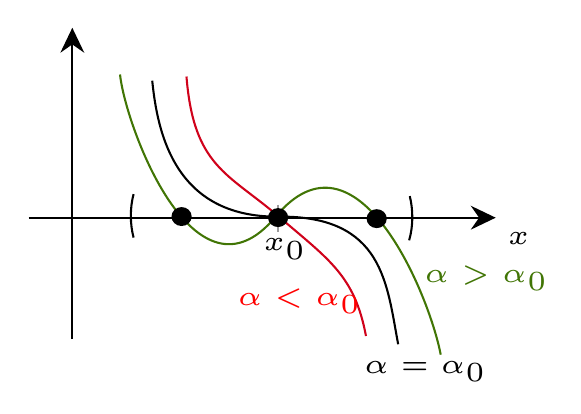
\begin{tikzpicture}[x=0.75pt,y=0.75pt,yscale=-1.5,xscale=1.5]
		%uncomment if require: \path (0,300); %set diagram left start at 0, and has height of 300
		
		%Straight Lines [id:da05892022845111411] 
		\draw    (217,100.67) -- (364,100.67) ;
		\draw [shift={(367,100.67)}, rotate = 180] [fill={rgb, 255:red, 0; green, 0; blue, 0 }  ][line width=0.08]  [draw opacity=0] (8.04,-3.86) -- (0,0) -- (8.04,3.86) -- (5.34,0) -- cycle    ;
		%Straight Lines [id:da806758973605693] 
		\draw    (231,139.67) -- (231,42.67) ;
		\draw [shift={(231,39.67)}, rotate = 90] [fill={rgb, 255:red, 0; green, 0; blue, 0 }  ][line width=0.08]  [draw opacity=0] (8.04,-3.86) -- (0,0) -- (8.04,3.86) -- (5.34,0) -- cycle    ;
		%Shape: Arc [id:dp6058068696964698] 
		\draw  [draw opacity=0] (250.68,107.06) .. controls (250.12,104.92) and (249.8,102.56) .. (249.8,100.07) .. controls (249.8,97.58) and (250.11,95.22) .. (250.68,93.1) -- (259.8,100.07) -- cycle ; \draw   (250.68,107.06) .. controls (250.12,104.92) and (249.8,102.56) .. (249.8,100.07) .. controls (249.8,97.58) and (250.11,95.22) .. (250.68,93.1) ;  
		%Shape: Arc [id:dp14042025356928334] 
		\draw  [draw opacity=0] (339.39,93.74) .. controls (339.91,95.81) and (340.2,98.08) .. (340.2,100.47) .. controls (340.2,103.14) and (339.84,105.68) .. (339.19,107.93) -- (330.2,100.47) -- cycle ; \draw   (339.39,93.74) .. controls (339.91,95.81) and (340.2,98.08) .. (340.2,100.47) .. controls (340.2,103.14) and (339.84,105.68) .. (339.19,107.93) ;  
		%Straight Lines [id:da25297557942373183] 
		\draw [color={rgb, 255:red, 155; green, 155; blue, 155 }  ,draw opacity=1 ]   (297.2,96.47) -- (297.2,105.27) ;
		%Curve Lines [id:da9485721249224925] 
		\draw [color={rgb, 255:red, 208; green, 2; blue, 27 }  ,draw opacity=1 ]   (267.67,55.33) .. controls (270,84.33) and (281,86.33) .. (297.33,100.33) .. controls (313.67,114.33) and (321.67,119.33) .. (325.33,138.67) ;
		%Curve Lines [id:da7115178345870963] 
		\draw [color={rgb, 255:red, 0; green, 0; blue, 0 }  ,draw opacity=1 ]   (256.67,56.67) .. controls (258.33,73) and (263.67,100.67) .. (297.33,100.33) .. controls (331,100) and (332,122) .. (335.67,141.33) ;
		%Curve Lines [id:da8498861454657496] 
		\draw [color={rgb, 255:red, 65; green, 117; blue, 5 }  ,draw opacity=1 ]   (246.33,54.67) .. controls (248,71) and (270.33,131.67) .. (296.33,100.33) .. controls (322.33,69) and (345.67,125.33) .. (349.33,144.67) ;
		%Shape: Path Data [id:dp508632932098046] 
		\draw  [fill={rgb, 255:red, 0; green, 0; blue, 0 }  ,fill opacity=1 ] (294.2,100.63) .. controls (294.2,99.14) and (295.5,97.93) .. (297.1,97.93) .. controls (298.7,97.93) and (300,99.14) .. (300,100.63) .. controls (300,102.12) and (298.7,103.33) .. (297.1,103.33) .. controls (295.5,103.33) and (294.2,102.12) .. (294.2,100.63) -- cycle ;
		%Shape: Path Data [id:dp4059785824642126] 
		\draw  [fill={rgb, 255:red, 0; green, 0; blue, 0 }  ,fill opacity=1 ] (263.2,100.3) .. controls (263.2,98.81) and (264.5,97.6) .. (266.1,97.6) .. controls (267.7,97.6) and (269,98.81) .. (269,100.3) .. controls (269,101.79) and (267.7,103) .. (266.1,103) .. controls (264.5,103) and (263.2,101.79) .. (263.2,100.3) -- cycle ;
		%Shape: Path Data [id:dp2560720790739939] 
		\draw  [fill={rgb, 255:red, 0; green, 0; blue, 0 }  ,fill opacity=1 ] (325.87,100.97) .. controls (325.87,99.48) and (327.17,98.27) .. (328.77,98.27) .. controls (330.37,98.27) and (331.67,99.48) .. (331.67,100.97) .. controls (331.67,102.46) and (330.37,103.67) .. (328.77,103.67) .. controls (327.17,103.67) and (325.87,102.46) .. (325.87,100.97) -- cycle ;
		
		% Text Node
		\draw (290.4,105.47) node [anchor=north west][inner sep=0.75pt]  [font=\tiny,xscale=2,yscale=2]  {$x_{0}$};
		% Text Node
		\draw (368.8,103.47) node [anchor=north west][inner sep=0.75pt]  [font=\tiny,xscale=2,yscale=2]  {$x$};
		% Text Node
		\draw (342,114.07) node [anchor=north west][inner sep=0.75pt]  [font=\tiny,color={rgb, 255:red, 65; green, 117; blue, 5 }  ,opacity=1 ,xscale=2,yscale=2]  {$\alpha  >\alpha _{0}$};
		% Text Node
		\draw (282,121.4) node [anchor=north west][inner sep=0.75pt]  [font=\tiny,color={rgb, 255:red, 255; green, 0; blue, 0 }  ,opacity=1 ,xscale=2,yscale=2]  {$\alpha < \alpha _{0}$};
		% Text Node
		\draw (322.67,144.73) node [anchor=north west][inner sep=0.75pt]  [font=\tiny,xscale=2,yscale=2]  {$\alpha =\alpha _{0}$};
		
		
	\end{tikzpicture}
\end{figure}

The dependence of $f(x,\alpha)$ on the variable $(x,\alpha)$ has the form $f(x,\alpha) = \xi_\alpha \xi_x - \xi_x^3$, where $\xi_\alpha = \alpha - \alpha_0$ and $\xi_x = x - x_0$.

Also, the following figure shows that branching diagram for the pitchfork bifurcation.
\begin{figure}[h!]
	\centering
	
	
	
	\tikzset{every picture/.style={line width=0.75pt}} %set default line width to 0.75pt        
	
	\begin{tikzpicture}[x=0.75pt,y=0.75pt,yscale=-1.5,xscale=1.5]
		%uncomment if require: \path (0,300); %set diagram left start at 0, and has height of 300
		
		%Straight Lines [id:da3228148192020939] 
		\draw    (181.33,188) -- (338.33,188) ;
		\draw [shift={(341.33,188)}, rotate = 180] [fill={rgb, 255:red, 0; green, 0; blue, 0 }  ][line width=0.08]  [draw opacity=0] (8.04,-3.86) -- (0,0) -- (8.04,3.86) -- (5.34,0) -- cycle    ;
		%Straight Lines [id:da35221396692761053] 
		\draw    (191.33,198) -- (191.33,51) ;
		\draw [shift={(191.33,48)}, rotate = 90] [fill={rgb, 255:red, 0; green, 0; blue, 0 }  ][line width=0.08]  [draw opacity=0] (8.04,-3.86) -- (0,0) -- (8.04,3.86) -- (5.34,0) -- cycle    ;
		%Shape: Arc [id:dp5974851327437227] 
		\draw  [draw opacity=0] (212.68,195.39) .. controls (212.12,193.26) and (211.8,190.89) .. (211.8,188.4) .. controls (211.8,185.92) and (212.11,183.56) .. (212.68,181.43) -- (221.8,188.4) -- cycle ; \draw   (212.68,195.39) .. controls (212.12,193.26) and (211.8,190.89) .. (211.8,188.4) .. controls (211.8,185.92) and (212.11,183.56) .. (212.68,181.43) ;  
		%Shape: Arc [id:dp5281588164715683] 
		\draw  [draw opacity=0] (310.72,181.41) .. controls (311.24,183.47) and (311.53,185.75) .. (311.53,188.13) .. controls (311.53,190.81) and (311.17,193.34) .. (310.52,195.6) -- (301.53,188.13) -- cycle ; \draw   (310.72,181.41) .. controls (311.24,183.47) and (311.53,185.75) .. (311.53,188.13) .. controls (311.53,190.81) and (311.17,193.34) .. (310.52,195.6) ;  
		%Straight Lines [id:da9580637116487603] 
		\draw [color={rgb, 255:red, 155; green, 155; blue, 155 }  ,draw opacity=1 ]   (261.53,183.13) -- (261.53,191.93) ;
		%Straight Lines [id:da580935466479485] 
		\draw [color={rgb, 255:red, 155; green, 155; blue, 155 }  ,draw opacity=1 ]   (185.67,118) -- (195.67,118) ;
		%Shape: Arc [id:dp8970538994160917] 
		\draw  [draw opacity=0] (198.51,166.65) .. controls (196.34,167.24) and (193.92,167.56) .. (191.37,167.57) .. controls (188.93,167.57) and (186.61,167.28) .. (184.51,166.75) -- (191.35,157.77) -- cycle ; \draw   (198.51,166.65) .. controls (196.34,167.24) and (193.92,167.56) .. (191.37,167.57) .. controls (188.93,167.57) and (186.61,167.28) .. (184.51,166.75) ;  
		%Shape: Arc [id:dp04436129064929517] 
		\draw  [draw opacity=0] (184.03,69.28) .. controls (186.15,68.68) and (188.51,68.33) .. (191,68.28) .. controls (193.49,68.24) and (195.85,68.52) .. (197.99,69.04) -- (191.17,78.28) -- cycle ; \draw   (184.03,69.28) .. controls (186.15,68.68) and (188.51,68.33) .. (191,68.28) .. controls (193.49,68.24) and (195.85,68.52) .. (197.99,69.04) ;  
		%Shape: Rectangle [id:dp11153113211033894] 
		\draw  [dash pattern={on 0.84pt off 2.51pt}] (211.53,68.27) -- (310.73,68.27) -- (310.73,168.27) -- (211.53,168.27) -- cycle ;
		%Curve Lines [id:da8104514892615617] 
		\draw    (261.13,118.27) .. controls (265.33,97.33) and (281.67,75.33) .. (306.97,70.3) ;
		%Curve Lines [id:da9062576670229996] 
		\draw    (306.67,164) .. controls (272.33,158) and (262.67,131) .. (261.13,118.27) ;
		%Curve Lines [id:da9563025736277584] 
		\draw  [dash pattern={on 4.5pt off 4.5pt}]  (261.13,118.27) .. controls (281.97,112.97) and (294.63,120.3) .. (310.97,116.97) ;
		%Curve Lines [id:da848406645414099] 
		\draw    (211.3,119.57) .. controls (232.13,114.27) and (244.8,121.6) .. (261.13,118.27) ;
		%Shape: Circle [id:dp46763773461044034] 
		\draw  [fill={rgb, 255:red, 208; green, 2; blue, 27 }  ,fill opacity=1 ] (259.27,117.9) .. controls (259.27,116.63) and (260.3,115.6) .. (261.57,115.6) .. controls (262.84,115.6) and (263.87,116.63) .. (263.87,117.9) .. controls (263.87,119.17) and (262.84,120.2) .. (261.57,120.2) .. controls (260.3,120.2) and (259.27,119.17) .. (259.27,117.9) -- cycle ;
		
		% Text Node
		\draw (342.33,200.4) node [anchor=north west][inner sep=0.75pt]  [font=\tiny,xscale=2,yscale=2]  {$\alpha $};
		% Text Node
		\draw (249.6,197) node [anchor=north west][inner sep=0.75pt]  [font=\tiny,xscale=2,yscale=2]  {$\alpha _{0}$};
		% Text Node
		\draw (176.4,115.33) node [anchor=north west][inner sep=0.75pt]  [font=\tiny,xscale=2,yscale=2]  {$x_{0}$};
		% Text Node
		\draw (174.73,43.67) node [anchor=north west][inner sep=0.75pt]  [font=\tiny,xscale=2,yscale=2]  {$x$};
		
		
	\end{tikzpicture}
\end{figure}

Again, we can intuitively figure out what conditions the functions $f(x,\alpha)$ should satisfy in order to have this kind of bifurcation.

\begin{enumerate}[(i)]
	\item $f(x-x_0,\alpha)$ be locally odd (in the neighborhood of $x_0$) with respect to $x$, i.e. $f(-(x-x_0),\alpha) = - f(x-x_0,\alpha)$ and $f(x_0,\alpha_0) =0 $. The local oddness also leads to 
	\begin{enumerate}[(a)]
		\item $f(x_0,\alpha) = 0$,
		\item $f_{xx}(x,\alpha)=0$, as well as any other even derivative.
	\end{enumerate} 
	\item $f_x(x_0,\alpha_0) =0$,
	\item $f_{xxx}(x_0,\alpha_0) \neq 0$,
	\item $f_{\alpha x} (x_0,\alpha_0) \neq 0$.
\end{enumerate}